\documentclass[11pt,a4paper]{article}
\usepackage[T1]{fontenc}
\usepackage[utf8]{inputenc}
\usepackage{lmodern}
\usepackage[margin=2.5cm]{geometry}
\usepackage{amsmath,amssymb}
\usepackage{graphicx}
\usepackage{float}
\usepackage{longtable,booktabs,array,calc}
\usepackage{microtype}
\usepackage{newunicodechar}
\usepackage{setspace}
\usepackage[hidelinks]{hyperref}
\usepackage{caption}
\captionsetup{font=small,labelfont=bf}
\setlength{\parskip}{4pt}
\setlength{\parindent}{0pt}
\setlength{\emergencystretch}{3em}
\newunicodechar{−}{\ensuremath{-}}
\newunicodechar{×}{\ensuremath{\times}}
\newunicodechar{₀}{\ensuremath{_0}}
\newunicodechar{χ}{\ensuremath{\chi}}
\newunicodechar{²}{\ensuremath{^2}}
\newunicodechar{≥}{\ensuremath{\geq}}
\newunicodechar{≤}{\ensuremath{\leq}}
\newunicodechar{…}{\ldots}
\newunicodechar{Δ}{\ensuremath{\Delta}}
\providecommand{\tightlist}{\setlength{\itemsep}{0pt}\setlength{\parskip}{0pt}}
\makeatletter
\def\fps@figure{H}
\makeatother

\title{Who saves from insulation? Persistent but unequal gas savings from cavity wall insulation in England and Wales}
\author{Kaustubh Ramekar\\[2pt]\small Independent researcher: technology, environment and society, London}
\date{10 November 2026}

\begin{document}
\maketitle

\begin{abstract}
\noindent ABSTRACT MISSING

\medskip
\noindent\textbf{Keywords:} 

\smallskip
\noindent\textbf{JEL:} Q41, Q48, C21, C23
\end{abstract}

\section*{2. Background}

Realised savings from insulation can fall well short of engineering predictions, and evidence on who saves least is thin and mixed. This section sets out that evidence, the closest prior study, and the methods the paper builds on.

\subsection*{2.1 Modelled versus realised savings}

The most cited ex post evidence is from the United States. Fowlie, Greenstone and Wolfram (2018) randomly encouraged take-up of the Weatherization Assistance Program and found that model-projected savings were more than three times realised savings. Allcott and Greenstone (2017) found that realised savings in a US utility programme were 68\% of the savings predicted to participants. Christensen, Francisco, Myers and Souza (2023) decomposed a similar gap. They attributed up to 41\% of it to bias in the engineering model, mainly for wall insulation, about 43\% to variation in workmanship, and only about 6\% to the rebound effect.

British evidence is closer to the engineering predictions. The Department of Energy and Climate Change (2014) compared insulated homes in NEED with matched uninsulated homes. It reported median gas savings of 9.2\% (1,500 kWh) for cavity wall insulation and 2.8\% (400 kWh) for loft insulation installed in 2011. Hamilton et al.~(2016) followed about 169,000 gas-heated English homes and found that retrofits reduced gas use, with larger reductions when measures were combined.

Webber, Gouldson and Kerr (2015) evaluated the Kirklees Warm Zone, which insulated about 51,000 homes in 2007--2010. Realised impacts exceeded predictions overall. In lower-income areas, though, impacts only matched predictions, while in middle- and higher-income areas they exceeded them. In the Netherlands, Kattenberg, Eichholtz and Kok (2026) found gas savings of about 19\% that persisted for up to ten years. Among owner-occupiers, higher-income households reduced gas use less than lower-income ones, the opposite of the Kirklees gradient.

\subsection*{2.2 Prebound, comfort-taking and warmth}

Two behavioural mechanisms can push realised savings below modelled savings. The \emph{prebound effect} (Sunikka-Blank and Galvin, 2012) is that homes with poor energy ratings use much less energy than their ratings predict, because occupants heat fewer rooms, for fewer hours, to lower temperatures. Such a home has less excess consumption to remove. Galvin and Sunikka-Blank (2016) argue that a large prebound effect combined with low income signals fuel poverty. \emph{Comfort-taking}, the direct rebound effect, is that occupants use part of an efficiency gain to heat their homes more (Sorrell, Dimitropoulos and Sommerville, 2009).

Both mechanisms are expected to be strongest in low-income households, who are more likely to under-heat to save money. Milne and Boardman (2000) analysed how much of the potential saving low-income households in monitored British schemes took back as higher temperatures, and how this depended on how warm the home was beforehand. In the Warm Front scheme, Hong, Oreszczyn and Ridley (2006) found that cavity wall and loft insulation reduced space-heating fuel use by about 10\% in centrally heated homes. In the Welsh Arbed scheme, Poortinga et al.~(2018) measured indoor temperatures about 0.84 K higher than in comparison homes after retrofit. Warmth matters for health: a Cochrane review found that warmth and energy efficiency improvements were associated with better general, respiratory and mental health, especially for people with inadequate warmth and chronic respiratory disease (Thomson et al., 2013).

Recent causal machine-learning evidence points the same way. D'Amico et al.~(2026) estimated much smaller savings from external wall insulation among English households with a high energy burden. Their consumption measure is modelled from the English Housing Survey rather than metered, so it cannot observe behaviour directly. The data used here are metered but contain no temperature measure. They can show who saves less gas, but not whether the difference is taken as warmth.

\subsection*{2.3 The closest prior study}

Peñasco and Díaz Anadón (2023) estimated dynamic effects of cavity wall and loft insulation on gas use in England and Wales. They used NEED data for about 55,000 households and gas years 2005--2017, and a dynamic difference-in-differences regression with household fixed effects, five leads and five lags. Cavity wall insulation cut gas use by about 6.9\% in the installation year. The effect became insignificant two years later, and the authors wrote that consumption returned to pre-installation levels after four years. They also found that gas use in the most deprived IMD band rose four and five years after installation. In a later comment, the authors clarified that savings fall rather than vanish, reporting cavity wall savings of 6--9\% after five years (Peñasco and Díaz Anadón, 2024).

This paper differs in four ways. First, it compares each installation cohort only with never-insulated homes, using an estimator that is robust to effects that differ across cohorts and over time. Second, it reports how sensitive the estimate is to violations of parallel trends rather than only testing for them. Third, it uses formal inference for heterogeneity, with a correction for multiple comparisons. Fourth, it uses the 2026 release of the public sample, with gas years to 2024, and publishes its code and logged specification. Section 5.2 tests directly whether a conventional fixed-effects specification on these data reproduces fading savings.

\subsection*{2.4 Methods}

The question ``what would this home's gas use have been without insulation?'' has a natural design in panel data: compare each home with itself before and after, against untreated homes over the same years (difference-in-differences). Its key assumption is parallel trends: without treatment, treated and comparison homes would have changed in the same way. Roth et al.~(2023) review recent work on this design.

Parallel trends is more plausible conditional on property characteristics. Sant'Anna and Zhao (2020) give a doubly robust estimator that is consistent if either a propensity model or an outcome model is correct. Chang (2020) shows how to fit those models with machine learning and cross-fitting, following Chernozhukov et al.~(2018). With staggered installation dates, comparing each cohort only with never-treated homes avoids the bias that two-way fixed effects estimators suffer when effects differ across cohorts (Callaway and Sant'Anna, 2021; Cengiz et al., 2019).

Two results guide the robustness analysis. Ding and Li (2019) show that difference-in-differences and adjustment for the lagged outcome bracket the true effect: if one of their identifying assumptions holds, the two estimates lie on either side of it. Rambachan and Roth (2023) show how to bound the effect when parallel trends fails by no more than a stated amount, judged against the violations seen before treatment.

For heterogeneity, causal forests (Wager and Athey, 2018; Athey, Tibshirani and Wager, 2019) estimate how the effect varies with covariates, but their individual estimates are noisy. Valid inference comes from three tools: the best linear projection of the conditional effect on chosen covariates (Semenova and Chernozhukov, 2021), group average treatment effects and classification analysis (GATES and CLAN; Chernozhukov et al., 2025), and the rank-weighted average treatment effect, which tests whether a ranking of units by predicted effect finds real differences (Yadlowsky et al., 2025).

\section*{3. Data}

The analysis uses the 50,000-home public sample of NEED, released by the Department for Energy Security and Net Zero (DESNZ) in June 2026 under the Open Government Licence (DESNZ, 2026a). The main sample has 1,801 homes with cavity wall insulation and 22,641 never-insulated comparison homes.

\subsection*{3.1 The NEED anonymised sample}

NEED links meter-point gas and electricity consumption to property attributes and to records of energy efficiency measures installed under government schemes. The public sample covers current domestic properties in England and Wales. For each home it gives annual gas and electricity use for 2005--2024, weather corrected and rounded to the nearest 100 kWh, with a validity flag for each year.

Flags mark each home that has had cavity wall insulation (CWI) or loft insulation (LI) through a scheme, with the year of installation. In the sample, 14.3\% of homes have a CWI record and 14.4\% an LI record; 53\% of the CWI and 72\% of the LI installations are dated 2007--2012. NEED does not record how much insulation a loft had before, and DECC's insulation statistics treated professional loft top-ups as a distinct category of scheme installation (DECC, 2012).

Gas years are not calendar years, and their definition changes during the period (DESNZ, 2026b):

\begin{longtable}[]{@{}ll@{}}
\toprule\noalign{}
Gas year & Period covered \\
\midrule\noalign{}
\endhead
\bottomrule\noalign{}
\endlastfoot
2005--2015 & October of the previous year to September \\
2016 & Mid-July 2016 to mid-July 2017 \\
2017 & Mid-June 2017 to mid-June 2018 \\
2018 onwards & Mid-May to mid-May of the following year \\
\end{longtable}

There is therefore a gap of about nine months between gas years 2015 and 2016, and gas years 2016--2018 overlap by about a month at each join. The main analysis window (Section 4.2) uses only gas years up to 2015 and is unaffected. In the event study, only the five-year coefficient for the 2011 cohort and the four- and five-year coefficients for the 2012 cohort use gas years 2016 and 2017. Weather correction applies in every year, though DESNZ notes that it does not fully adjust for rapid, extreme weather changes.

Property variables are type, age band, floor area band, council tax band, Energy Performance Certificate (EPC) band and region. Area deprivation is given as the quintile of the English or Welsh Index of Multiple Deprivation (IMD) for the home's small area. The public sample has no postcode or small-area code, and no tenure or income variable.

\subsection*{3.2 Sample construction}

\begin{enumerate}
\def\labelenumi{\arabic{enumi}.}
\tightlist
\item
  \textbf{Gas-heated homes.} Homes whose main heating fuel is gas (40,445 of 50,000).
\item
  \textbf{Treated homes.} CWI recorded in 2007--2012, with no loft insulation recorded in the six-year window around it. Loft-only homes, defined the same way, form a second treatment group.
\item
  \textbf{Comparison homes.} Gas-heated homes with neither CWI nor LI ever recorded.
\item
  \textbf{Valid consumption.} A home enters a cohort only if its gas use is flagged valid in all four years of that cohort's window (Section 4.2).
\end{enumerate}

\begin{longtable}[]{@{}ll@{}}
\toprule\noalign{}
Group & Homes \\
\midrule\noalign{}
\endhead
\bottomrule\noalign{}
\endlastfoot
CWI only, installed 2007--2012 & 1,801 \\
Loft insulation only, installed 2007--2012 & 2,877 \\
Never insulated (comparison) & 22,641 \\
Stacked home-cohort rows, CWI analysis & 106,019 \\
\end{longtable}

Of the 1,801 CWI homes, 83 are in Wales. Before installation, CWI homes used a median of 16,300 kWh of gas a year, against 15,300 kWh for comparison homes.

\subsection*{3.3 Selection into treatment}

Uptake was not random. CWI was most common in the most and least deprived IMD quintiles (about 18\% and 17\% of homes) and fell with council tax band, from 17\% in band A to 5\% in band G. Only 5\% of homes built before 1930 received it, against 20--24\% of homes built in 1930--99, because most older homes have solid walls with no cavity. Appendix A reports the resulting imbalance and how far the estimator's weights remove it.

\section*{4. Empirical design}

The estimand is the average effect of insulation on the gas use of insulated homes (the average treatment effect on the treated, ATT), estimated by comparing each home's change in gas use with that of similar never-insulated homes.

\subsection*{4.1 Stacked cohorts}

Homes insulated in each year g from 2007 to 2012 form a cohort. Each cohort is paired with all never-insulated homes, and the six cohort datasets are stacked (Cengiz et al., 2019). Comparison homes therefore appear once per cohort, and inference is clustered by home. Comparing treated homes only with never-treated homes avoids using already-treated homes as controls, which biases two-way fixed effects estimates when effects differ by cohort or over time.

\subsection*{4.2 Timing and outcome}

Pre-installation years are g−2 and g−1; post-installation years are g+2 and g+3. Years g and g+1 are left out. Before 2015, gas years run October to September, while installation dates are calendar years, so an installation late in year g can fall in gas year g+1.

The outcome is the change in mean log gas use between the two windows:

\[
\Delta Y_{ig} = \tfrac{1}{2}\left(\ln y_{i,g+2} + \ln y_{i,g+3}\right) - \tfrac{1}{2}\left(\ln y_{i,g-2} + \ln y_{i,g-1}\right)
\]

Effects are in log points; the percentage saving is 1 − exp(ATT).

\subsection*{4.3 Doubly robust difference-in-differences}

Let D be 1 for a treated home and 0 for a comparison home, and X the covariates. Two nuisance functions are estimated: the propensity p(X) = P(D = 1 \textbar{} X) and the comparison-group outcome model m₀(X) = E{[}ΔY \textbar{} D = 0, X{]}. The doubly robust ATT (Sant'Anna and Zhao, 2020) with normalised weights is:

\[
\widehat{\mathrm{ATT}} = \frac{\sum_i D_i\,(\Delta Y_i - \hat m_0(X_i))}{\sum_i D_i} \;-\; \frac{\sum_i w_i\,(\Delta Y_i - \hat m_0(X_i))}{\sum_i w_i}, \qquad w_i = \frac{(1-D_i)\,\hat p(X_i)}{1-\hat p(X_i)}
\]

It is consistent if either nuisance model is correct. Both are fitted with gradient-boosted trees and five-fold cross-fitting, with folds grouped by home so a home's own data never fits its own predictions (Chang, 2020; Chernozhukov et al., 2018). Fitted propensities are clipped to {[}0.01, 0.99{]}. Standard errors come from the estimator's influence function, summed within homes.

Machine learning has a narrow job here. It fits the two nuisance functions flexibly, so that the analyst does not have to choose interactions between property type, age, size, region and deprivation by hand. Identification still rests on conditional parallel trends, which no learner can supply.

\subsection*{4.4 Covariates and the baseline-gas problem}

All covariates are fixed before installation: property type, age band, floor area band, council tax band (bands G--I merged), IMD quintile with a nation indicator, region, cohort, and mean log gas use over the pre-installation years g−2 and g−1.

EPC band is excluded. It is mostly recorded after installation and reflects the insulation itself, so conditioning on it would absorb part of the effect. Council tax band is based on 1991 property values, so insulation cannot have changed it; it serves as a proxy for property value and household wealth in the absence of tenure or income.

The gas covariate needs care. It is built from the same years, g−2 and g−1, that form the pre-period of the outcome. A home with a temporarily high reading in those years will tend to fall back afterwards whether or not it is insulated (regression to the mean). Adjusting for that reading turns the design into a hybrid of difference-in-differences and adjustment for the lagged outcome. Ding and Li (2019) show that these two approaches bracket the true effect when either one's assumption holds. The main specification, committed before the outcomes were analysed, keeps this covariate. Section 5.1 reports it alongside three alternatives:

\begin{enumerate}
\def\labelenumi{\arabic{enumi}.}
\tightlist
\item
  \textbf{Pure difference-in-differences:} no gas covariate.
\item
  \textbf{Lagged-outcome adjustment:} the outcome is post-period mean log gas, adjusting for the pre-period level, with no differencing.
\item
  \textbf{Earlier baseline:} the gas covariate is built from g−4 and g−3, outside the outcome window. Because gas data start in 2005, this is possible only for the 2009--2012 cohorts. On those cohorts, the same-window and no-covariate versions are re-estimated for a like-for-like comparison.
\end{enumerate}

\subsection*{4.5 Heterogeneity and multiple comparisons}

One heterogeneity question was committed in advance: are savings smaller in IMD quintile 1 than in quintile 5? Subgroup ATTs by IMD quintile use the same nuisance fits, with the estimator restricted to that subgroup. The standard error of the Q1−Q5 gap allows for comparison homes shared between the two estimates. All other subgroup analyses, by council tax band and property age, are exploratory. For the three contrasts reported (IMD Q1 against Q5, council tax band A against bands D--F, and homes built in 1930--72 against 1973--99), p-values are also given with Holm's adjustment. The minimum detectable effect at 80\% power and a 5\% two-sided test is 2.80 times the standard error of each contrast.

Three further tools give valid inference on heterogeneity.

\begin{enumerate}
\def\labelenumi{\arabic{enumi}.}
\tightlist
\item
  \textbf{Best linear projection (BLP).} The conditional effect among treated homes is projected on IMD quintile, council tax band, floor area band, age band and baseline log gas, using the doubly robust score with home-clustered sandwich standard errors (Semenova and Chernozhukov, 2021). With the covariates Z centred on treated means, the intercept is the ATT:
\end{enumerate}

\[
\hat\beta = \Big(\sum_i D_i Z_i Z_i^{\top}\Big)^{-1} \sum_i \Big(D_i - (1-D_i)\frac{\hat p(X_i)}{1-\hat p(X_i)}\Big) Z_i \big(\Delta Y_i - \hat m_0(X_i)\big)
\]

The projection is run on the main sample, with the same-window baseline, and on the 2009--2012 cohorts with the earlier baseline from g−4 and g−3.

\begin{enumerate}
\def\labelenumi{\arabic{enumi}.}
\setcounter{enumi}{1}
\tightlist
\item
  \textbf{GATES and CLAN.} Homes are split at random into two halves, by home. A causal forest (CausalForestDML; Battocchi et al., 2019) with 400 trees is fitted to one half and used to rank the other half by predicted saving. On the held-out half, the doubly robust ATT is estimated within terciles of that ranking (GATES), and the mean characteristics of treated homes in the top and bottom terciles are compared (CLAN). The forest's heterogeneity variables are IMD quintile, council tax band, age band, floor area band, property type and same-window baseline log gas; region, nation and cohort are controls. This is repeated over 20 random splits. Each split gives estimates with 97.5\% confidence intervals; the reported estimate and bounds are the medians across splits, and the reported p-value is twice the median p-value, which preserves 95\% coverage (Chernozhukov et al., 2025).
\item
  \textbf{Targeting test (AUTOC).} On each held-out half, the saving among the top fraction q of treated homes ranked by the forest (with comparison homes above the same score threshold) is compared with the saving among all homes. The area under this targeting curve, averaged over q = 0.1, 0.2, \ldots, 1.0, measures whether the ranking finds real differences; it is zero if it does not. This adapts the rank-weighted average treatment effect of Yadlowsky et al.~(2025) to the ATT. Standard errors come from 300 home-level Bayesian bootstrap draws with the nuisance fits held fixed, and splits are combined as above.
\end{enumerate}

\subsection*{4.6 Checks and transparency}

\begin{enumerate}
\def\labelenumi{\arabic{enumi}.}
\tightlist
\item
  \textbf{Event study.} The same estimator applied to the change from year g−1 to each year g+e, for e from −4 to +5. The joint covariance of the nine coefficients comes from home-level influence functions, which allows a joint test of the pre-installation coefficients and the sensitivity analysis in Section 4.7.
\item
  \textbf{Robustness.} Post years g+1 and g+2; outcome in kWh levels; loft insulation as the treatment; propensities clipped at 0.001 instead of 0.01; rows with propensity below 0.01 trimmed rather than clipped; and pre-1930 homes excluded.
\item
  \textbf{Placebo outcome.} Electricity use, which wall insulation should barely affect in gas-heated homes.
\item
  \textbf{Comparison with a conventional specification.} A two-way fixed effects regression of log gas on home and year fixed effects and event-time indicators from −5 to +5, on gas years 2005--2017, mirroring the design of Peñasco and Díaz Anadón (2023). It is run on all gas-heated homes, with separate indicators for cavity wall and loft insulation, and on the units of the main design only.
\end{enumerate}

The main specification (sample, timing, outcome, covariates, estimator and the IMD question) was written down and committed to version control before any consumption values were analysed. Every later change, including all of the analyses in Sections 4.4, 4.5 and 4.7 beyond the main specification, is logged with its date and reason in the repository (deviations D1--D12). This is not a formal pre-registration, because the specification was not registered with a third party.

\subsection*{4.7 Sensitivity to parallel-trends violations}

A pre-installation coefficient that differs from zero does not by itself show that parallel trends fails after installation, and one that is close to zero does not show that it holds (Roth et al., 2023). Following Rambachan and Roth (2023), I instead ask how large a post-installation violation would have to be to overturn the conclusion that insulation saves gas.

The target is the average of the event-study coefficients two and three years after installation, the same post-installation years as the main estimate. Two restrictions are used. Under \emph{relative magnitudes}, the change in the violation between consecutive post-installation years is at most \(\bar{M}\) times the largest such change before installation. Under \emph{smoothness}, the slope of the violation can change by at most M log points per year. For each value, the robust 95\% confidence set is computed with the Python port of Rambachan and Roth's method (\texttt{honestdid} 0.1.1), using conditional least-favourable intervals for relative magnitudes and fixed-length intervals for smoothness. The breakdown value is the smallest \(\bar{M}\) or M at which the confidence set includes zero.

The target differs from the main 8.8\% estimate in two ways: its base year is g−1 alone, and it has no gas covariate. The sensitivity analysis therefore bounds the event-study analogue of the main estimate, not the 8.8\% itself.

\section*{5. Results}

Cavity wall insulation reduced gas use by 8.8\% (95\% CI 7.5--10.2\%), or 1,437 kWh a year (1,262--1,612 kWh). The saving appears in the installation year and holds for five years, and the estimate changes little across specifications that handle the baseline, overlap and timing differently.

\subsection*{5.1 Average effects}

\textbf{Table 1.} Effect of cavity wall insulation (CWI) on gas use. Saving = 1 − exp(ATT); home-clustered 95\% confidence intervals.

\begin{longtable}[]{@{}
  >{\raggedright\arraybackslash}p{(\columnwidth - 8\tabcolsep) * \real{0.5114}}
  >{\raggedright\arraybackslash}p{(\columnwidth - 8\tabcolsep) * \real{0.0795}}
  >{\raggedright\arraybackslash}p{(\columnwidth - 8\tabcolsep) * \real{0.1364}}
  >{\raggedright\arraybackslash}p{(\columnwidth - 8\tabcolsep) * \real{0.1250}}
  >{\raggedright\arraybackslash}p{(\columnwidth - 8\tabcolsep) * \real{0.1477}}@{}}
\toprule\noalign{}
\begin{minipage}[b]{\linewidth}\raggedright
Specification
\end{minipage} & \begin{minipage}[b]{\linewidth}\raggedright
Cohorts
\end{minipage} & \begin{minipage}[b]{\linewidth}\raggedright
Gas saving
\end{minipage} & \begin{minipage}[b]{\linewidth}\raggedright
95\% CI
\end{minipage} & \begin{minipage}[b]{\linewidth}\raggedright
Treated homes
\end{minipage} \\
\midrule\noalign{}
\endhead
\bottomrule\noalign{}
\endlastfoot
\textbf{Main specification} (committed in advance) & 2007--12 & 8.8\% & 7.5--10.2 & 1,801 \\
Pure DiD: no gas covariate & 2007--12 & 10.6\% & 9.2--12.0 & 1,801 \\
Lagged-outcome adjustment & 2007--12 & 9.0\% & 7.6--10.3 & 1,801 \\
Early baseline covariate (g−4, g−3) & 2009--12 & 9.7\% & 8.0--11.3 & 1,143 \\
Same-window covariate, same cohorts & 2009--12 & 9.1\% & 7.4--10.7 & 1,143 \\
Pure DiD, same cohorts & 2009--12 & 10.2\% & 8.5--11.9 & 1,143 \\
Post years g+1 to g+2 & 2007--12 & 9.6\% & 8.4--10.7 & 1,757 \\
Outcome in kWh & 2007--12 & 1,437 kWh/yr & 1,262--1,612 & 1,801 \\
Propensities clipped at 0.001 & 2007--12 & 8.8\% & 7.5--10.1 & 1,801 \\
Pre-1930 homes excluded & 2007--12 & 8.9\% & 7.5--10.3 & 1,670 \\
Propensity below 0.01 trimmed & 2007--12 & 8.9\% & 7.5--10.3 & 1,647 \\
Loft insulation only (second treatment) & 2007--12 & 2.4\% & 1.2--3.7 & 2,877 \\
Placebo: CWI effect on electricity & 2007--12 & 0.2\% & −1.4 to 1.8 & 1,991 \\
\end{longtable}

The main estimate is close to DESNZ's matched-comparison estimate for 2011 installations, 9.2\% or 1,500 kWh (Department of Energy and Climate Change, 2014), despite a different estimator and sample.

The baseline covariate moves the estimate, but only within a narrow range. Without it (pure difference-in-differences) the saving is 10.6\%; with lagged-outcome adjustment instead of differencing it is 9.0\%. If either approach's assumption holds, these two bracket the true effect (Ding and Li, 2019), so the saving lies between about 9.0\% and 10.6\%. The main estimate, 8.8\%, sits just below that range, so it is, if anything, conservative. On the 2009--2012 cohorts, replacing the same-window covariate with one built from g−4 and g−3 raises the estimate from 9.1\% to 9.7\%. Regression to the mean in the baseline covariate therefore does not inflate the average saving; if anything it slightly lowers it.

\subsection*{5.2 Timing}

\begin{figure}[H]\centering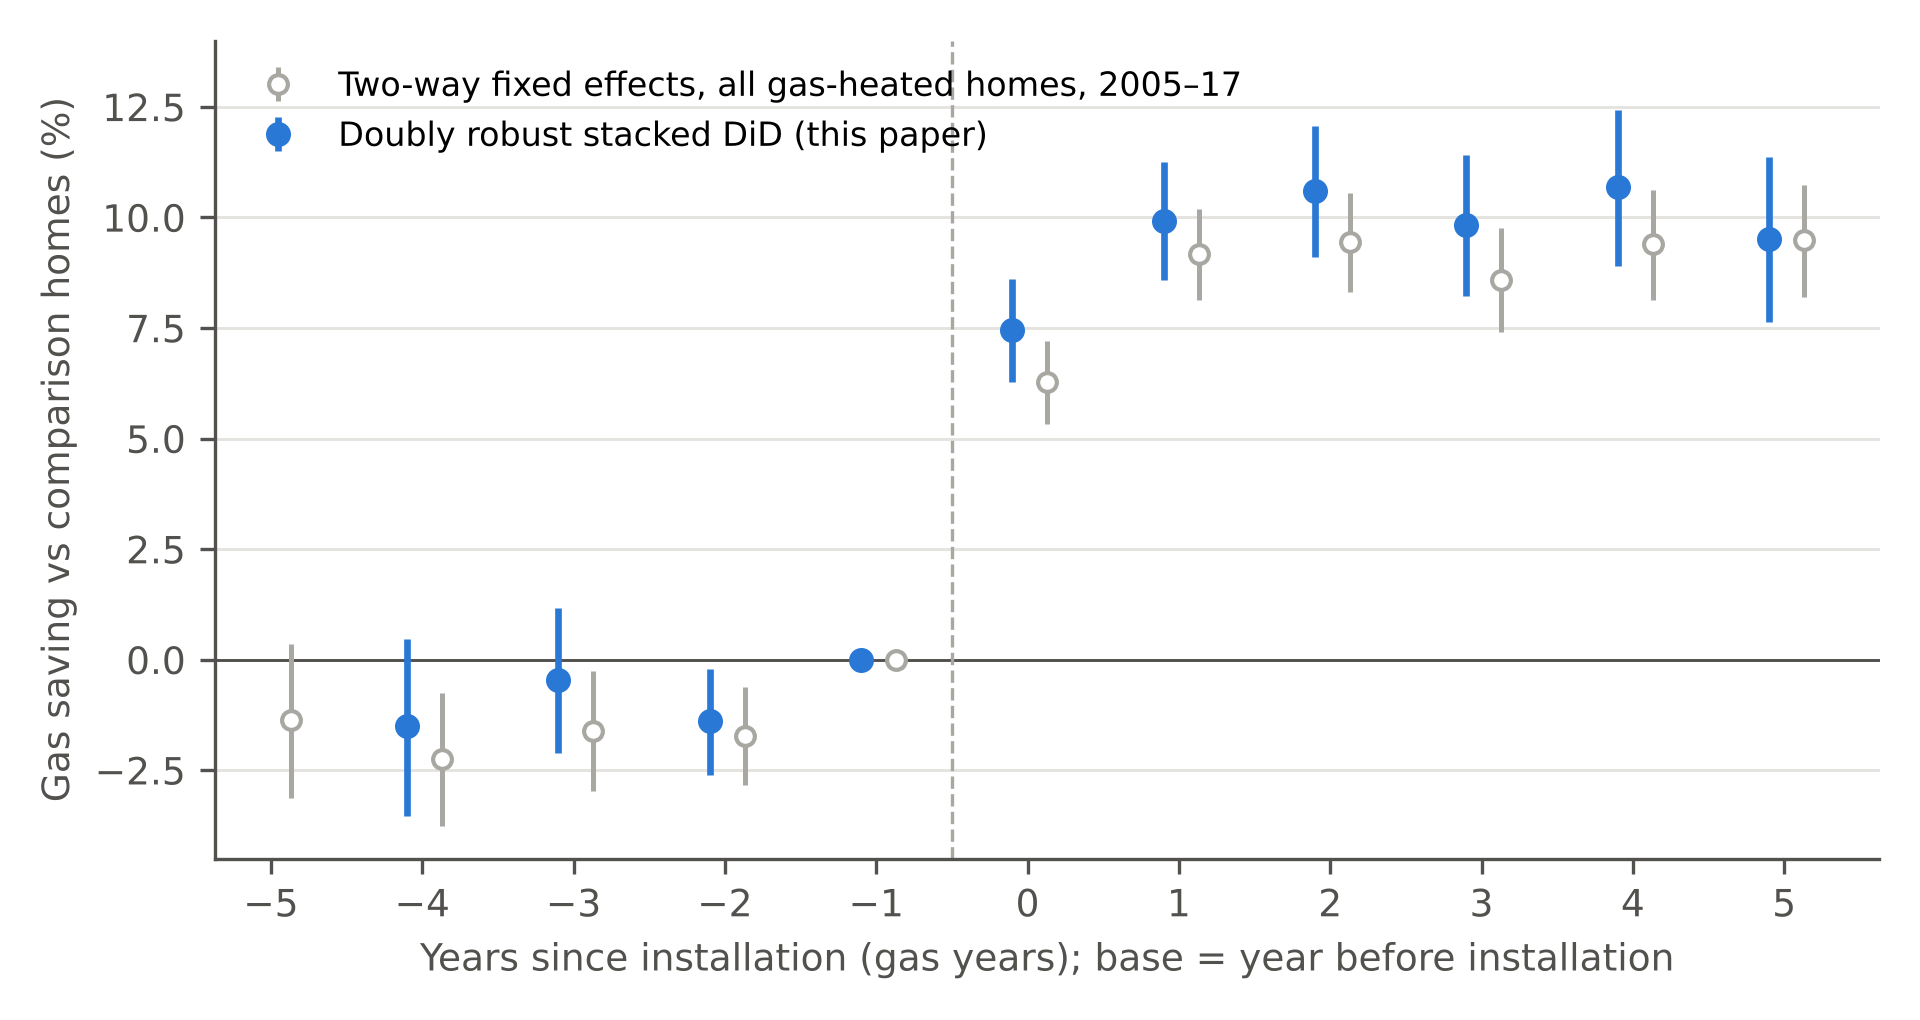
\includegraphics[width=\linewidth]{figures/fig1_event_study.png}\caption{NEED anonymised data 2026 (DESNZ). Blue: doubly robust stacked DiD, 1,367–2,003 treated homes per year, home-clustered 95\% CIs. Grey: two-way fixed effects on all gas-heated homes, gas years 2005–2017.\textbackslash{}}\label{fig:event}\end{figure}

Savings reach 7.5\% in the installation gas year, which includes months before installation, and about 10--11\% from the first full year. Over years one to five they average 10.1\%, and five years on they are still 9.5\%, with no sign of decay.

\textbf{Reconciling 8.8\% and 10\%.} The main estimate (8.8\%) and the event-study level (about 10\%) differ mainly because the main estimate adjusts for pre-installation gas use and the event study does not; the main estimate without that covariate is 10.6\%. Their different base years (the mean of g−2 and g−1 against g−1 alone) matter less.

Before installation, the estimates are small. Two years before, treated homes used 1.4\% more gas relative to comparison homes than in the base year (95\% CI 0.2--2.6\%). Three and four years before, the differences are 0.5\% and 1.5\% and not significant. The three pre-installation coefficients are not jointly significant (Wald χ² = 6.55 with 3 degrees of freedom, p = 0.088).

A conventional two-way fixed effects regression on these data also shows no fading (Figure 1, grey; Appendix Table C1). On all gas-heated homes, with separate indicators for loft insulation, savings are 9.2--9.5\% in years one, two, four and five and 8.6\% in year three. On the units of the main design only, they are 9.9--10.9\% in years one to five. The fading savings reported by Peñasco and Díaz Anadón (2023) are therefore not reproduced on the 2026 public sample by either estimator (Section 7.2).

\subsection*{5.3 Sensitivity to parallel-trends violations}

\textbf{Table 2.} Robust 95\% confidence sets for the average saving two and three years after installation (Rambachan and Roth, 2023). The target uses g−1 as base year and no gas covariate.

\begin{longtable}[]{@{}
  >{\raggedright\arraybackslash}p{(\columnwidth - 8\tabcolsep) * \real{0.3839}}
  >{\raggedright\arraybackslash}p{(\columnwidth - 8\tabcolsep) * \real{0.1429}}
  >{\raggedright\arraybackslash}p{(\columnwidth - 8\tabcolsep) * \real{0.1071}}
  >{\raggedright\arraybackslash}p{(\columnwidth - 8\tabcolsep) * \real{0.2500}}
  >{\raggedright\arraybackslash}p{(\columnwidth - 8\tabcolsep) * \real{0.1161}}@{}}
\toprule\noalign{}
\begin{minipage}[b]{\linewidth}\raggedright
Restriction on post-installation violations
\end{minipage} & \begin{minipage}[b]{\linewidth}\raggedright
Value
\end{minipage} & \begin{minipage}[b]{\linewidth}\raggedright
Estimate (\%)
\end{minipage} & \begin{minipage}[b]{\linewidth}\raggedright
Robust 95\% CI for saving (\%)
\end{minipage} & \begin{minipage}[b]{\linewidth}\raggedright
Includes zero
\end{minipage} \\
\midrule\noalign{}
\endhead
\bottomrule\noalign{}
\endlastfoot
None (parallel trends holds exactly) & -- & 10.2 & 8.8--11.6 & No \\
Relative magnitudes & \(\bar{M}\) = 0.5 & & 5.7--14.3 & No \\
Relative magnitudes & \(\bar{M}\) = 1 & & 1.6--15.1 & No \\
Relative magnitudes & \(\bar{M}\) = 1.25 & & −0.5 to 15.1 & Yes \\
Relative magnitudes & \(\bar{M}\) = 1.5 & & −2.7 to 15.1 & Yes \\
Smoothness & M = 0 & & 6.3--11.8 & No \\
Smoothness & M = 0.0025 & & 3.8--13.3 & No \\
Smoothness & M = 0.005 & & 0.8--14.8 & No \\
Smoothness & M = 0.0075 & & −2.2 to 16.1 & Yes \\
\end{longtable}

The conclusion that insulation saves gas survives post-installation violations of parallel trends as large as the largest violation seen before installation (\(\bar{M}\) = 1). It breaks down between \(\bar{M}\) = 1 and \(\bar{M}\) = 1.25. Under the smoothness restriction, a linear trend extrapolated from the pre-period (M = 0) still leaves a saving of 6.3--11.8\%. The conclusion survives if the slope of that trend changes by up to 0.5 percentage points a year (M = 0.005), and breaks down by 0.75.

The breakdown values show that the qualitative finding is robust to violations of the size the pre-period shows, but not much larger ones. The size of the saving is less certain than its sign: at \(\bar{M}\) = 1 the robust interval runs from 1.6\% to 15.1\%.

\subsection*{5.4 Robustness and placebo}

Shifting the post window one year earlier gives 9.6\%, close to the event-study level. The three overlap checks (clipping at 0.001, trimming rows below 0.01, and excluding pre-1930 homes) all give 8.8--8.9\%. Loft insulation saved 2.4\%, close to DESNZ's 2.8\%.

Electricity use, which wall insulation should not much affect in gas-heated homes, shows no change (0.2\%, CI −1.4 to 1.8\%). This argues against the result being driven by other changes in treated households, such as occupancy, that would move all energy use together.

\section*{6. Who saves least}

Savings were smallest in the lowest-value homes: 5.0\% in council tax band A against 11.0\% in bands D--F, a gap that survives correction for multiple comparisons. The gap by area deprivation is smaller and not statistically significant. Pre-retrofit gas use, measured outside the outcome window, does not explain either.

\subsection*{6.1 Subgroup effects}

\begin{figure}[H]\centering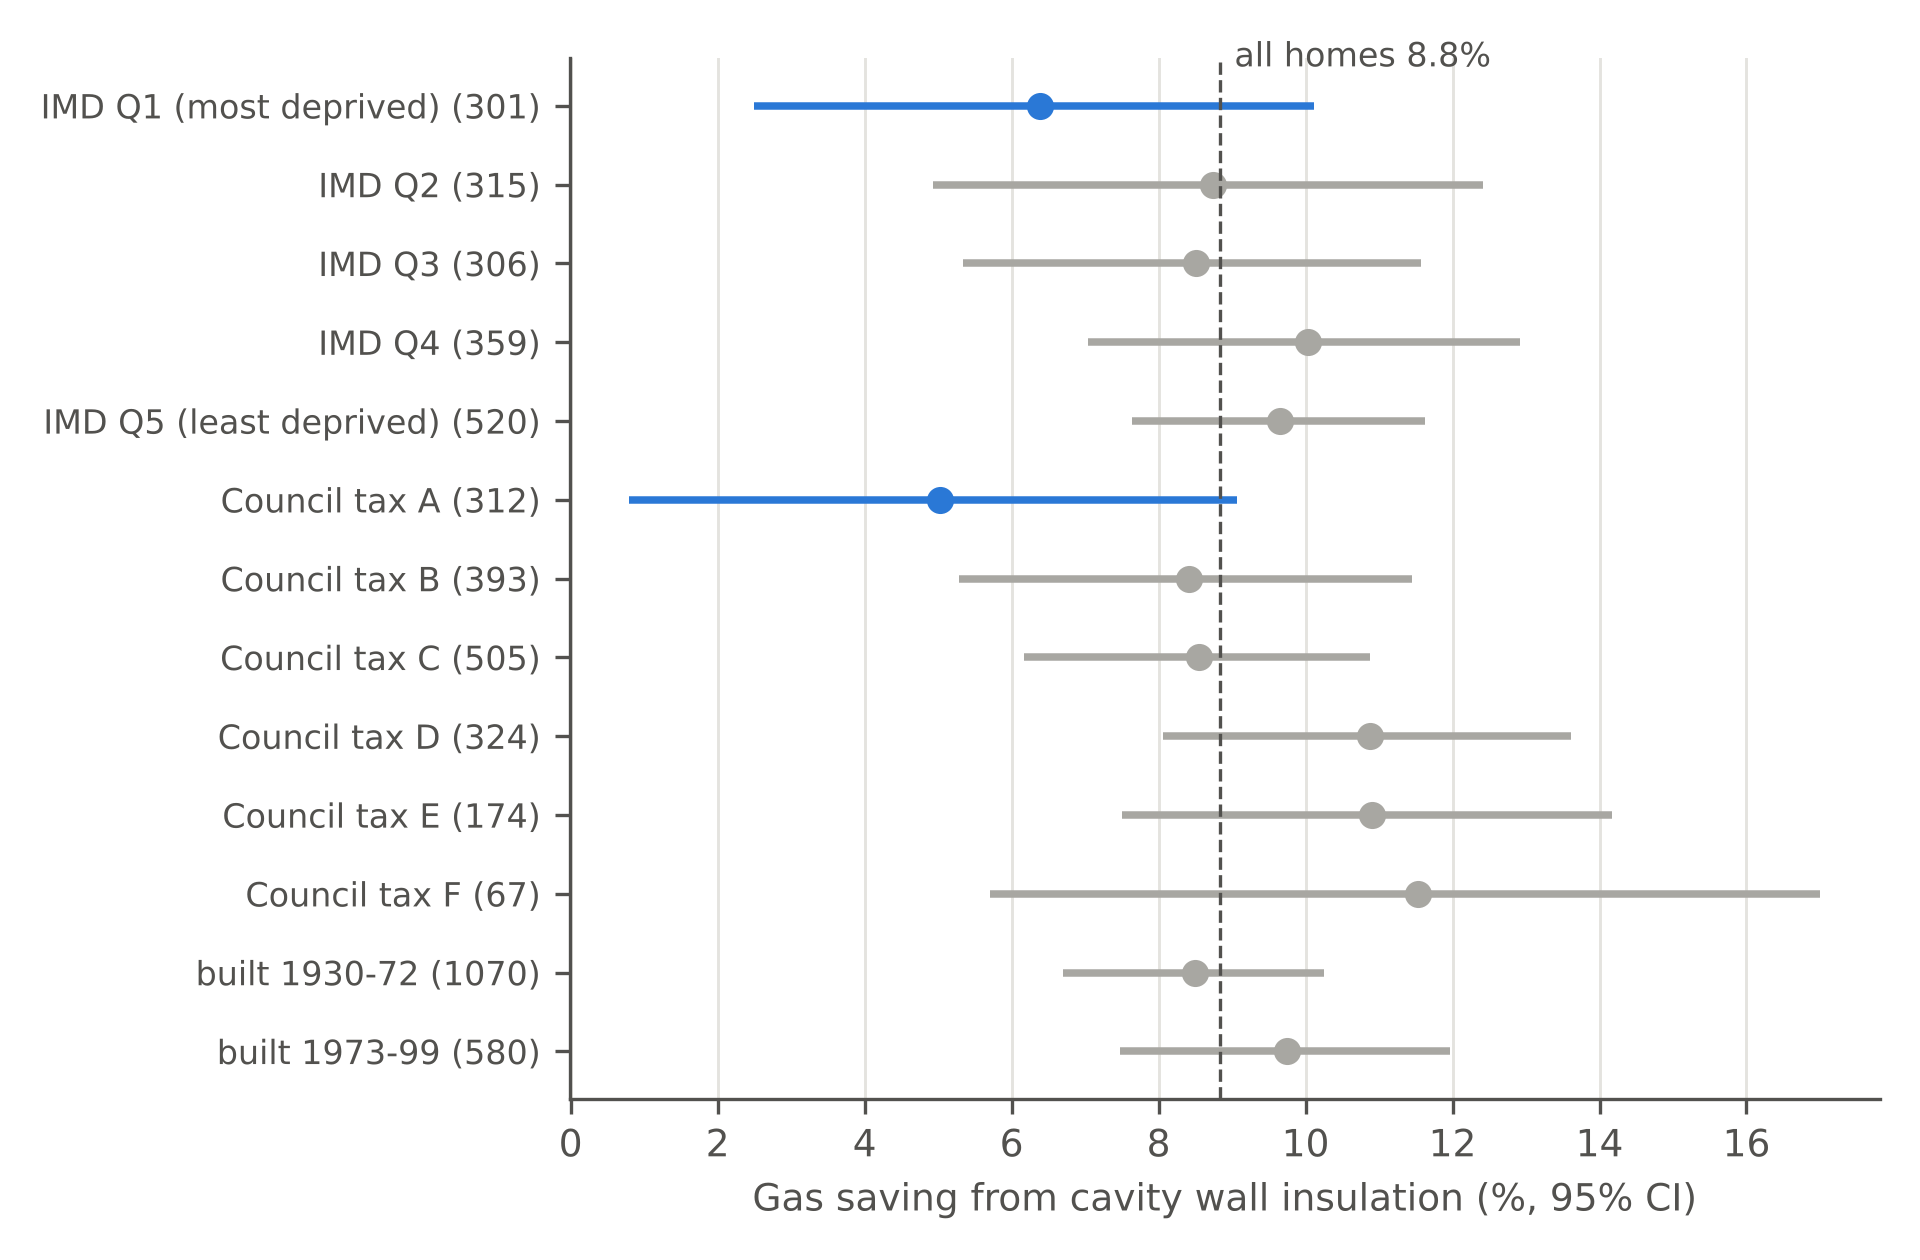
\includegraphics[width=\linewidth]{figures/fig2_subgroups.png}\caption{NEED anonymised data 2026 (DESNZ). CWI homes installed 2007–12; doubly robust DiD within subgroup, home-clustered 95\% CIs. Subgroups other than IMD quintile are exploratory.\textbackslash{}}\label{fig:subgroups}\end{figure}

Across IMD quintiles, savings rise from 6.4\% in the most deprived to 9.7--10.0\% in the two least deprived. The gap between quintiles 1 and 5, the one heterogeneity test committed in advance, is 3.6 log points (95\% CI −1.1 to 8.2, p = 0.13). The minimum gap the sample could detect with 80\% power is 6.6 log points, nearly twice the gap observed. The data are therefore consistent both with no deprivation gap and with one of up to about 8 log points.

The gradient by council tax band is steeper: 5.0\% in band A, 8.4--8.6\% in bands B and C, and 10.9--11.5\% in bands D to F. Homes built in 1973--99 save slightly more than those built in 1930--72 (9.7\% against 8.5\%). Table 3 tests the three contrasts.

\textbf{Table 3.} Differences in saving between subgroups (log points × 100). Holm-adjusted p-values cover the three contrasts; MDE is the minimum detectable gap at 80\% power and 5\% two-sided significance.

\begin{longtable}[]{@{}
  >{\raggedright\arraybackslash}p{(\columnwidth - 12\tabcolsep) * \real{0.4096}}
  >{\raggedright\arraybackslash}p{(\columnwidth - 12\tabcolsep) * \real{0.1325}}
  >{\raggedright\arraybackslash}p{(\columnwidth - 12\tabcolsep) * \real{0.0723}}
  >{\raggedright\arraybackslash}p{(\columnwidth - 12\tabcolsep) * \real{0.1325}}
  >{\raggedright\arraybackslash}p{(\columnwidth - 12\tabcolsep) * \real{0.0723}}
  >{\raggedright\arraybackslash}p{(\columnwidth - 12\tabcolsep) * \real{0.0723}}
  >{\raggedright\arraybackslash}p{(\columnwidth - 12\tabcolsep) * \real{0.1084}}@{}}
\toprule\noalign{}
\begin{minipage}[b]{\linewidth}\raggedright
Contrast
\end{minipage} & \begin{minipage}[b]{\linewidth}\raggedright
Savings (\%)
\end{minipage} & \begin{minipage}[b]{\linewidth}\raggedright
Gap
\end{minipage} & \begin{minipage}[b]{\linewidth}\raggedright
95\% CI
\end{minipage} & \begin{minipage}[b]{\linewidth}\raggedright
p
\end{minipage} & \begin{minipage}[b]{\linewidth}\raggedright
Holm p
\end{minipage} & \begin{minipage}[b]{\linewidth}\raggedright
MDE (80\%)
\end{minipage} \\
\midrule\noalign{}
\endhead
\bottomrule\noalign{}
\endlastfoot
IMD Q1 − Q5 (committed in advance) & 6.4 vs 9.7 & 3.6 & −1.1 to 8.2 & 0.132 & 0.265 & 6.6 \\
Council tax A − bands D--F & 5.0 vs 11.0 & 6.5 & 1.6--11.4 & 0.010 & 0.029 & 7.0 \\
Built 1930--72 − built 1973--99 & 8.5 vs 9.7 & 1.4 & −1.8 to 4.5 & 0.390 & 0.390 & 4.5 \\
\end{longtable}

The council-tax gap is 6.5 log points (95\% CI 1.6--11.4) and remains significant after Holm's adjustment (p = 0.029). Because it was not specified in advance, it should be read as a strong exploratory finding rather than a confirmed one. The age-band gap is small and not significant.

Council tax band is closely tied to property type. Among treated homes, 70\% of those in band A are flats or terraced houses, against 7\% in bands D--F, where 52\% are detached. Section 6.4 asks whether the gradient survives holding property type fixed.

\subsection*{6.2 Pre-retrofit gas use}

The first version of this analysis found that pre-installation gas use was the strongest predictor of savings in a causal forest. It read this as support for the prebound effect: homes that used little gas had less to save. That baseline, however, was the mean of g−2 and g−1, the same years that form the pre-period of the outcome. Readings in those years carry temporary ups and downs that fall back afterwards whether or not a home is insulated. If insulated homes were more often treated after a spell of unusually high use, those with high readings would fall back further than comparison homes with the same readings, and would appear to save more. That pattern is regression to the mean, not prebound.

Table 4 removes the overlap by measuring baseline use in g−4 and g−3, two years before the outcome window, for the 2009--2012 cohorts.

\textbf{Table 4.} Savings by tercile of earlier gas use (g−4, g−3), CWI homes installed 2009--12.

\begin{longtable}[]{@{}
  >{\raggedright\arraybackslash}p{(\columnwidth - 12\tabcolsep) * \real{0.2679}}
  >{\raggedright\arraybackslash}p{(\columnwidth - 12\tabcolsep) * \real{0.1964}}
  >{\raggedright\arraybackslash}p{(\columnwidth - 12\tabcolsep) * \real{0.0893}}
  >{\raggedright\arraybackslash}p{(\columnwidth - 12\tabcolsep) * \real{0.0893}}
  >{\raggedright\arraybackslash}p{(\columnwidth - 12\tabcolsep) * \real{0.1339}}
  >{\raggedright\arraybackslash}p{(\columnwidth - 12\tabcolsep) * \real{0.1071}}
  >{\raggedright\arraybackslash}p{(\columnwidth - 12\tabcolsep) * \real{0.1161}}@{}}
\toprule\noalign{}
\begin{minipage}[b]{\linewidth}\raggedright
Tercile of gas use in g−4, g−3
\end{minipage} & \begin{minipage}[b]{\linewidth}\raggedright
Mean baseline (kWh/yr)
\end{minipage} & \begin{minipage}[b]{\linewidth}\raggedright
Saving (\%)
\end{minipage} & \begin{minipage}[b]{\linewidth}\raggedright
95\% CI (\%)
\end{minipage} & \begin{minipage}[b]{\linewidth}\raggedright
Saving (kWh/yr)
\end{minipage} & \begin{minipage}[b]{\linewidth}\raggedright
95\% CI (kWh)
\end{minipage} & \begin{minipage}[b]{\linewidth}\raggedright
Treated homes
\end{minipage} \\
\midrule\noalign{}
\endhead
\bottomrule\noalign{}
\endlastfoot
Lowest & 10,503 & 10.5 & 7.2--13.7 & 975 & 643--1,307 & 381 \\
Middle & 17,232 & 8.3 & 5.6--10.9 & 1,262 & 882--1,643 & 379 \\
Highest & 26,302 & 10.2 & 7.5--12.8 & 2,173 & 1,697--2,648 & 383 \\
\end{longtable}

The proportional saving shows no gradient: 10.5\%, 8.3\% and 10.2\% from the lowest to the highest tercile. The saving in kWh rises roughly in proportion to prior use. Homes that used little gas before saved about the same share as homes that used a lot.

This contradicts the simplest version of the prebound account, in which low users save a smaller share. It does not rule out prebound altogether. Low total use reflects home size and occupancy as well as under-heating, and the public sample holds no modelled demand against which under-heating could be measured.

\subsection*{6.3 Causal forest}

The first-version causal forest estimated an average effect of 8.9\% for treated homes, close to the main estimate. Its variable importance ranked same-window baseline gas use first (0.44), then property age (0.20), council tax band (0.14), IMD quintile (0.10) and floor area (0.06). Variable importance records how often the forest splits on a variable, not whether the effect truly differs along it. The top-ranked variable is also the one most exposed to regression to the mean.

A single held-out split in the first version gave savings of 10.6\%, 9.0\% and 6.7\% across terciles of predicted saving. One split is a noisy basis for inference, so Section 6.4 replaces it with repeated splits and formal tests.

\section*{7. Discussion}

Three conclusions are well supported. Scheme-installed cavity wall insulation cut gas use by about 9--10\%. The saving lasted at least five years. It was smaller in the lowest-value homes. A fourth, the reason for that gradient, remains open.

\subsection*{7.1 Interpreting the property-value gradient}

Savings in council tax band A homes were about half those in bands D--F. Four explanations fit this, and the data can rule out only one.

\begin{enumerate}
\def\labelenumi{\arabic{enumi}.}
\tightlist
\item
  \textbf{Prebound, proxied by low prior gas use.} If band A homes save less because they used little gas before, savings should fall with prior use. Measured outside the outcome window, they do not (Section 6.2). Total gas use is a weak proxy for under-heating, though, because it also reflects home size and occupancy. A direct test needs modelled demand before the retrofit, which the public sample does not hold.
\item
  \textbf{Comfort-taking.} Households may use part of the improvement to keep warmer. This lowers measured savings most where homes were coldest, and fits evidence from monitored British schemes (Milne and Boardman, 2000; Poortinga et al., 2018). The data contain no temperature measure, so it cannot be tested here.
\item
  \textbf{Installation quality.} Christensen et al.~(2023) attribute much of the gap between projected and realised savings to variation in workmanship. Cavities in cheaper housing may be harder to fill fully, or more often partly filled already. NEED does not record either.
\item
  \textbf{Building physics.} Band A homes are more often small terraced houses and flats, with less exposed wall per unit of floor area. Property type and floor area enter the nuisance models, but floor area is recorded only in coarse bands, and property type is not among the projection covariates in Section 6.4.
\end{enumerate}

These explanations carry different welfare implications. Under comfort-taking, a smaller gas saving comes with a gain in warmth, which is associated with better health for people in cold homes (Thomson et al., 2013). Under poor installation, it is simply a smaller benefit. The data cannot tell these apart.

Council tax band measures property value in 1991, not household income. Band A includes much social housing, whose tenants are often on low incomes, and some owner-occupiers who are not. The gradient is therefore one by property value, not proven to be one by income.

\subsection*{7.2 Why savings persist here but faded in earlier NEED work}

Peñasco and Díaz Anadón (2023) found cavity wall savings that faded within a few years. Here they do not. The obvious suspect is the estimator, since fixed-effects regressions with staggered treatment can produce misleading dynamics when effects vary across cohorts (Roth et al., 2023). On these data, however, a conventional fixed-effects specification also shows no fading (Figure 1 and Appendix Table C1). The difference is therefore unlikely to come from the estimator alone.

It may come from the data release, since the earlier study used gas years only to 2017 from an earlier NEED release, or from sample construction, covariates or the treatment of homes with several measures. The public files do not allow an exact replication, so this question stays open. The fixed-effects specification on all gas-heated homes does show pre-installation coefficients of 1.4--2.3\%, three of them significant, larger than in the main design. That is a reminder that results from this kind of regression on NEED depend on who is in the comparison group.

Persistence is consistent with evidence from other settings. In the Netherlands, Kattenberg, Eichholtz and Kok (2026) found insulation savings that lasted up to ten years.

\subsection*{7.3 Implications for scheme scoring and fuel poverty}

The Energy Company Obligation credits suppliers with modelled savings, not metered ones. ECO3 deemed scores were built from SAP and RdSAP modelling of typical dwellings, and their methodology notes that the score for a measure ``is unlikely to match the actual saving'' of a given installation (Ofgem, 2018). ECO4 scores rest on modelled annual bill savings and the home's post-project SAP rating (Ofgem, 2026).

Two findings bear on this. First, the average cavity wall saving held for at least five years, so these data give no reason to shorten the lifetime over which savings are credited. Second, measured savings were about half as large in band A homes as in bands D--F. If two homes of the same archetype receive the same score, the score will overstate the realised gas saving in the lower-value home relative to the other. This paper does not compare realised savings with deemed scores directly, because the public sample does not contain them.

The official fuel-poverty measure in England, Low Income Low Energy Efficiency (LILEE), already avoids metered use. A household is fuel poor if its home has a fuel-poverty energy efficiency rating of band D or below and its income after modelled energy costs falls below the poverty line. Those costs are modelled at an adequate heating regime, because fuel-poor households may limit their energy use (DESNZ, 2026c). Insulation can therefore move a home out of LILEE fuel poverty even when its metered gas use falls little.

For scheme evaluation, the implication is narrow but concrete. Metered kWh saved measures one benefit of a retrofit. Where households under-heated before, it may understate progress on the fuel-poverty measure the schemes target. This paper shows only the smaller kWh saving, not any warmth or health gain. Measuring those requires temperature or health data alongside meter readings.

\subsection*{7.4 Threats to the design}

\begin{itemize}
\tightlist
\item
  \textbf{Parallel trends.} Two years before installation, treated homes used 1.4\% more gas relative to comparison homes than in the base year. The three pre-installation coefficients are not jointly significant (p = 0.088). Savings remain significant unless violations after installation exceed those before it (Section 5.3).
\item
  \textbf{Contaminated comparison group.} NEED records only measures installed through government schemes. Some comparison homes were probably insulated privately, which would bias the estimates towards zero. The savings here are best read as lower bounds.
\item
  \textbf{Selection on unobservables.} Households that took up insulation may differ in ways the covariates miss, such as changes in occupancy. Differencing removes fixed differences between homes, and the electricity placebo argues against broad household changes, but neither rules out shocks specific to heating.
\item
  \textbf{Overlap.} Weighting removes most, but not all, of the covariate imbalance; pre-1930 homes remain over-represented among weighted comparison homes (Appendix A). Results are similar when propensities are clipped differently, trimmed, or pre-1930 homes are dropped (Table 1).
\item
  \textbf{Spatial correlation.} Standard errors are clustered by home. Schemes were often delivered area by area, and the public sample has no small-area code, so errors that are correlated within areas cannot be accounted for. Confidence intervals may be somewhat too narrow.
\item
  \textbf{Measurement.} Consumption is annual, weather corrected and rounded to 100 kWh, and the gas-year definition changes during the period (Section 3.1). These add noise but apply equally to treated and comparison homes.
\item
  \textbf{Survivorship and fuel.} The sample contains only properties that still exist and are matched to meters in 2025, and main heating fuel is defined from 2022--2024 consumption. Insulation is unlikely to change either.
\end{itemize}

\subsection*{7.5 What the public sample cannot do}

The public file has no tenure, income or small-area code. The study therefore cannot compare social renters, private renters and owner-occupiers, although tenure is central to retrofit policy. Social landlords deliver much retrofit, and private renters face the split incentive between landlord and tenant. With about 300 treated homes per IMD quintile, the sample also lacks the power to detect a deprivation gap of the size observed. The much larger licensed NEED file, available through the UK Data Service, would address both.

\section*{8. Conclusion}

Cavity wall insulation installed under government schemes in 2007--2012 cut gas use in gas-heated homes in England and Wales by 8.8\% in the main specification, about 1,440 kWh a year, and by 9.0--10.6\% across the bracketing specifications. The saving appeared in the installation year and showed no sign of fading over five years, under both the main estimator and a conventional fixed-effects specification.

Savings were not equal. They were about half as large in council tax band A homes as in bands D--F, a gap that survives correction for multiple comparisons. The gap by area deprivation was smaller and not statistically significant, and the sample could not have detected a gap of that size. Low gas use before the retrofit, measured outside the outcome window, does not explain who saved least. An apparent link in a first analysis came from regression to the mean.

Why lower-value homes save less remains open. Comfort-taking, installation quality and building physics all fit the evidence, and metered gas data alone cannot separate them. Repeating the analysis on the licensed NEED file would add tenure and the power to study deprivation. Linking meter data to indoor temperatures would show whether smaller savings in poorer homes are a loss or a gain in warmth.

\section*{Data and code availability}

All code, the main specification with its dated deviation log (D1--D12), result tables, figures and this paper's LaTeX source are at \href{https://github.com/TheAlchemist108/insulation-causal}{github.com/TheAlchemist108/insulation-causal}. The data are the NEED anonymised data 2026, 50,000-row sample, published by DESNZ under the Open Government Licence v3.0; its download URL and SHA-256 hash are recorded in the repository.

The analysis used Python 3.13 with NumPy, pandas, SciPy, scikit-learn 1.9, EconML 0.17, statsmodels and honestdid 0.1.1; exact versions are in \texttt{requirements.txt}. The random seed is 20261106. The main pipeline runs in about 15 minutes on a laptop; the repeated-split heterogeneity analysis takes about an hour.

\section*{Use of AI tools}

The author used Claude (Anthropic), a large language model, as a research assistant for this study: to help write and debug the analysis code, search and check the literature, and draft and edit text. All analyses were run on the public data with the code in the repository, and the author reviewed the code, results and text and takes full responsibility for them.

\section*{Competing interests and funding}

The author declares no competing interests. This work received no specific funding.

\section*{References}

\begin{list}{}{\setlength{\leftmargin}{1.5em}\setlength{\itemindent}{-1.5em}\setlength{\itemsep}{2pt}}
\tightlist
\item
  Allcott, H. and Greenstone, M. (2012). Is there an energy efficiency gap? \emph{Journal of Economic Perspectives} 26(1), 3--28.
\item
  Allcott, H. and Greenstone, M. (2017). Measuring the welfare effects of residential energy efficiency programs. NBER Working Paper 23386 (revised January 2024).
\item
  Athey, S., Tibshirani, J. and Wager, S. (2019). Generalized random forests. \emph{Annals of Statistics} 47(2), 1148--1178.
\item
  Battocchi, K., Dillon, E., Hei, M., Lewis, G., Oka, P., Oprescu, M. and Syrgkanis, V. (2019). EconML: A Python package for ML-based heterogeneous treatment effects estimation. github.com/py-why/EconML.
\item
  Callaway, B. and Sant'Anna, P. H. C. (2021). Difference-in-differences with multiple time periods. \emph{Journal of Econometrics} 225(2), 200--230.
\item
  Cengiz, D., Dube, A., Lindner, A. and Zipperer, B. (2019). The effect of minimum wages on low-wage jobs. \emph{Quarterly Journal of Economics} 134(3), 1405--1454.
\item
  Chang, N.-C. (2020). Double/debiased machine learning for difference-in-differences models. \emph{The Econometrics Journal} 23(2), 177--191.
\item
  Chernozhukov, V., Chetverikov, D., Demirer, M., Duflo, E., Hansen, C., Newey, W. and Robins, J. (2018). Double/debiased machine learning for treatment and structural parameters. \emph{The Econometrics Journal} 21(1), C1--C68.
\item
  Chernozhukov, V., Demirer, M., Duflo, E. and Fernández-Val, I. (2025). Fisher--Schultz lecture: Generic machine learning inference on heterogeneous treatment effects in randomized experiments, with an application to immunization in India. \emph{Econometrica} 93(4), 1121--1164.
\item
  Christensen, P., Francisco, P., Myers, E. and Souza, M. (2023). Decomposing the wedge between projected and realized returns in energy efficiency programs. \emph{Review of Economics and Statistics} 105(4), 798--817.
\item
  D'Amico, B., Pomponi, F., Arehart, J. H. and Khaddour, L. (2026). Who cuts emissions, who turns up the heat? Causal machine learning estimates of energy efficiency interventions. \emph{Energy and Buildings} 350, 116613.
\item
  Department of Energy and Climate Change (2012). Changes to insulation statistics methodology. London: DECC. {[}VERIFY: the document is undated; it describes changes implemented in the September 2012 statistical release.{]}
\item
  Department of Energy and Climate Change (2014). National Energy Efficiency Data-Framework: Summary of analysis using the National Energy Efficiency Data-Framework (NEED). London: DECC, June 2014.
\item
  Department for Energy Security and Net Zero (2026a). National Energy Efficiency Data-Framework (NEED): anonymised data 2026. London: DESNZ. Open Government Licence v3.0.
\item
  Department for Energy Security and Net Zero (2026b). Domestic NEED 2026 Annex D: methodology note. London: DESNZ.
\item
  Department for Energy Security and Net Zero (2026c). Fuel poverty statistics: methodology handbook 2026. London: DESNZ.
\item
  Ding, P. and Li, F. (2019). A bracketing relationship between difference-in-differences and lagged-dependent-variable adjustment. \emph{Political Analysis} 27(4), 605--615.
\item
  Fowlie, M., Greenstone, M. and Wolfram, C. (2018). Do energy efficiency investments deliver? Evidence from the Weatherization Assistance Program. \emph{Quarterly Journal of Economics} 133(3), 1597--1644.
\item
  Galvin, R. and Sunikka-Blank, M. (2016). Quantification of (p)rebound effects in retrofit policies: Why does it matter? \emph{Energy} 95, 415--424.
\item
  Hamilton, I. G., Summerfield, A. J., Shipworth, D., Steadman, J. P., Oreszczyn, T. and Lowe, R. J. (2016). Energy efficiency uptake and energy savings in English houses: A cohort study. \emph{Energy and Buildings} 118, 259--276.
\item
  Hong, S. H., Oreszczyn, T., Ridley, I. and the Warm Front Study Group (2006). The impact of energy efficient refurbishment on the space heating fuel consumption in English dwellings. \emph{Energy and Buildings} 38(10), 1171--1181.
\item
  Kattenberg, L., Eichholtz, P. and Kok, N. (2026). The efficacy of energy efficiency: Measuring the returns to home insulation. \emph{Energy Economics} 158, 109366.
\item
  Milne, G. and Boardman, B. (2000). Making cold homes warmer: The effect of energy efficiency improvements in low-income homes. \emph{Energy Policy} 28(6--7), 411--424.
\item
  Ofgem (2018). ECO3 deemed scores methodology. Report prepared by BRE. London: Ofgem.
\item
  Ofgem (2026). ECO4 scores. ofgem.gov.uk/guidance/eco4-scores, accessed 10 November 2026.
\item
  Peñasco, C. and Díaz Anadón, L. (2023). Assessing the effectiveness of energy efficiency measures in the residential sector gas consumption through dynamic treatment effects: Evidence from England and Wales. \emph{Energy Economics} 117, 106435.
\item
  Peñasco, C. and Díaz Anadón, L. (2024). A comment on ``Assessing the effectiveness of energy efficiency measures in the residential sector gas consumption through dynamic treatment effects: Evidence from England and Wales''. \emph{Energy Economics} 139, 107946.
\item
  Poortinga, W., Jiang, S., Grey, C. and Tweed, C. (2018). Impacts of energy-efficiency investments on internal conditions in low-income households. \emph{Building Research \& Information} 46(6), 653--667.
\item
  Quispe, A. (2026). honestdid: Robust inference in difference-in-differences and event study designs (Python package, version 0.1.1, released 3 March 2026). github.com/anzonyquispe/honestdid.
\item
  Rambachan, A. and Roth, J. (2023). A more credible approach to parallel trends. \emph{Review of Economic Studies} 90(5), 2555--2591.
\item
  Roth, J., Sant'Anna, P. H. C., Bilinski, A. and Poe, J. (2023). What's trending in difference-in-differences? A synthesis of the recent econometrics literature. \emph{Journal of Econometrics} 235(2), 2218--2244.
\item
  Sant'Anna, P. H. C. and Zhao, J. (2020). Doubly robust difference-in-differences estimators. \emph{Journal of Econometrics} 219(1), 101--122.
\item
  Semenova, V. and Chernozhukov, V. (2021). Debiased machine learning of conditional average treatment effects and other causal functions. \emph{The Econometrics Journal} 24(2), 264--289.
\item
  Sorrell, S., Dimitropoulos, J. and Sommerville, M. (2009). Empirical estimates of the direct rebound effect: A review. \emph{Energy Policy} 37(4), 1356--1371.
\item
  Sunikka-Blank, M. and Galvin, R. (2012). Introducing the prebound effect: The gap between performance and actual energy consumption. \emph{Building Research \& Information} 40(3), 260--273.
\item
  Thomson, H., Thomas, S., Sellstrom, E. and Petticrew, M. (2013). Housing improvements for health and associated socio-economic outcomes. \emph{Cochrane Database of Systematic Reviews} 2013, Issue 2, CD008657.
\item
  Wager, S. and Athey, S. (2018). Estimation and inference of heterogeneous treatment effects using random forests. \emph{Journal of the American Statistical Association} 113(523), 1228--1242.
\item
  Webber, P., Gouldson, A. and Kerr, N. (2015). The impacts of household retrofit and domestic energy efficiency schemes: A large scale, ex post evaluation. \emph{Energy Policy} 84, 35--43.
\item
  Yadlowsky, S., Fleming, S., Shah, N., Brunskill, E. and Wager, S. (2025). Evaluating treatment prioritization rules via rank-weighted average treatment effects. \emph{Journal of the American Statistical Association} 120(549), 38--51.
\end{list}

\section*{Appendix A. Covariate balance and overlap}

Raw comparison homes differ from treated homes mainly in age, type and region. Of 46 covariate columns, 22 have an absolute standardised mean difference (SMD) above 0.1 before weighting, the largest being pre-1930 homes (−0.59). With the estimator's comparison-group weights p/(1−p), 5 remain above 0.1 and the largest is −0.24, again pre-1930 homes. The outcome model of the doubly robust estimator adjusts for the remaining differences, and excluding pre-1930 homes leaves the estimate unchanged (8.9\%; Table 1).

\textbf{Table A1.} Means and standardised mean differences for selected covariates (stacked rows; comparison rows weighted by p/(1−p)). All 46 columns are in \texttt{outputs/revision/balance.csv}.

\begin{longtable}[]{@{}
  >{\raggedright\arraybackslash}p{(\columnwidth - 10\tabcolsep) * \real{0.3333}}
  >{\raggedright\arraybackslash}p{(\columnwidth - 10\tabcolsep) * \real{0.1212}}
  >{\raggedright\arraybackslash}p{(\columnwidth - 10\tabcolsep) * \real{0.1515}}
  >{\raggedright\arraybackslash}p{(\columnwidth - 10\tabcolsep) * \real{0.2020}}
  >{\raggedright\arraybackslash}p{(\columnwidth - 10\tabcolsep) * \real{0.0707}}
  >{\raggedright\arraybackslash}p{(\columnwidth - 10\tabcolsep) * \real{0.1212}}@{}}
\toprule\noalign{}
\begin{minipage}[b]{\linewidth}\raggedright
Covariate
\end{minipage} & \begin{minipage}[b]{\linewidth}\raggedright
Treated mean
\end{minipage} & \begin{minipage}[b]{\linewidth}\raggedright
Comparison, raw
\end{minipage} & \begin{minipage}[b]{\linewidth}\raggedright
Comparison, weighted
\end{minipage} & \begin{minipage}[b]{\linewidth}\raggedright
SMD raw
\end{minipage} & \begin{minipage}[b]{\linewidth}\raggedright
SMD weighted
\end{minipage} \\
\midrule\noalign{}
\endhead
\bottomrule\noalign{}
\endlastfoot
Built before 1930 & 0.073 & 0.289 & 0.162 & −0.59 & −0.24 \\
Built 1930--72 & 0.594 & 0.430 & 0.533 & 0.33 & 0.12 \\
Built 1973--99 & 0.322 & 0.232 & 0.278 & 0.20 & 0.10 \\
Built 2000 or later & 0.011 & 0.049 & 0.027 & −0.22 & −0.10 \\
Mid terrace & 0.120 & 0.235 & 0.164 & −0.30 & −0.12 \\
Semi-detached & 0.389 & 0.279 & 0.355 & 0.23 & 0.07 \\
Flat & 0.098 & 0.146 & 0.109 & −0.15 & −0.03 \\
Detached & 0.199 & 0.153 & 0.176 & 0.12 & 0.06 \\
North West & 0.243 & 0.114 & 0.205 & 0.34 & 0.10 \\
London & 0.061 & 0.159 & 0.097 & −0.32 & −0.12 \\
IMD quintile 1 & 0.167 & 0.188 & 0.173 & −0.05 & −0.01 \\
IMD quintile 5 & 0.289 & 0.222 & 0.261 & 0.15 & 0.06 \\
Council tax band A & 0.173 & 0.209 & 0.180 & −0.09 & −0.02 \\
Council tax band D & 0.180 & 0.172 & 0.176 & 0.02 & 0.01 \\
Pre-period mean ln gas (g−2, g−1) & 9.651 & 9.566 & 9.637 & 0.16 & 0.03 \\
Floor area band 1 (smallest) & 0.066 & 0.097 & 0.072 & −0.11 & −0.02 \\
Floor area band 4 & 0.031 & 0.058 & 0.045 & −0.13 & −0.07 \\
\end{longtable}

Propensities are low throughout, because treated homes are few relative to stacked comparison rows. The median fitted propensity is 0.026 for treated homes and 0.014 for comparison rows; the maximum is 0.14 for treated homes. The clipping floor of 0.01 binds for 8.6\% of treated rows and 38\% of comparison rows. Clipping at 0.001 instead, or trimming rows below 0.01, leaves the estimate at 8.8--8.9\% (Table 1).

\textbf{Table A2.} Quantiles of the fitted propensity (main specification, clipped at 0.01).

\begin{longtable}[]{@{}lll@{}}
\toprule\noalign{}
Quantile & Treated rows & Comparison rows \\
\midrule\noalign{}
\endhead
\bottomrule\noalign{}
\endlastfoot
0.00 & 0.0100 & 0.0100 \\
0.05 & 0.0100 & 0.0100 \\
0.25 & 0.0168 & 0.0100 \\
0.50 & 0.0263 & 0.0136 \\
0.75 & 0.0372 & 0.0241 \\
0.95 & 0.0607 & 0.0452 \\
0.99 & 0.0826 & 0.0672 \\
1.00 & 0.1358 & 0.2781 \\
\end{longtable}

\section*{Appendix B. Minimum detectable effects}

For a contrast with standard error SE, the minimum detectable gap at 80\% power and a 5\% two-sided test is (1.96 + 0.84) × SE = 2.80 × SE. The IMD Q1 − Q5 contrast has SE = 0.0236 log points, so its MDE is 0.066 log points (6.6 percentage points of saving, approximately). The observed gap, 0.036, is a little over half that. The council-tax contrast (SE 0.0250) has an MDE of 0.070, and its observed gap, 0.065, is close to it. The age contrast (SE 0.0161) has an MDE of 0.045.

In the first two cases the subgroups have about 300--570 treated homes each. Detecting a deprivation gap of 3.6 log points with 80\% power would need standard errors about 45\% smaller, more than three times as many treated homes per quintile.

\section*{Appendix C. Event-study coefficients}

\textbf{Table C1.} Saving relative to the gas year before installation (\%; negative values mean treated homes used more gas than in the base year). This paper: doubly robust stacked DiD with home-clustered 95\% CIs. Two-way FE: home and year fixed effects, event-time indicators −5 to +5 with endpoints binned, gas years 2005--2017, standard errors clustered by home; ``all homes'' uses 419,160 home-years from 38,384 gas-heated homes with separate loft-insulation indicators, and ``main-design units'' uses 313,148 home-years from 29,329 homes.

\begin{longtable}[]{@{}
  >{\raggedright\arraybackslash}p{(\columnwidth - 10\tabcolsep) * \real{0.0438}}
  >{\raggedright\arraybackslash}p{(\columnwidth - 10\tabcolsep) * \real{0.1606}}
  >{\raggedright\arraybackslash}p{(\columnwidth - 10\tabcolsep) * \real{0.0876}}
  >{\raggedright\arraybackslash}p{(\columnwidth - 10\tabcolsep) * \real{0.0949}}
  >{\raggedright\arraybackslash}p{(\columnwidth - 10\tabcolsep) * \real{0.2774}}
  >{\raggedright\arraybackslash}p{(\columnwidth - 10\tabcolsep) * \real{0.3358}}@{}}
\toprule\noalign{}
\begin{minipage}[b]{\linewidth}\raggedright
Year e
\end{minipage} & \begin{minipage}[b]{\linewidth}\raggedright
This paper: saving (\%)
\end{minipage} & \begin{minipage}[b]{\linewidth}\raggedright
95\% CI
\end{minipage} & \begin{minipage}[b]{\linewidth}\raggedright
Treated homes
\end{minipage} & \begin{minipage}[b]{\linewidth}\raggedright
Two-way FE, all homes: saving (95\% CI)
\end{minipage} & \begin{minipage}[b]{\linewidth}\raggedright
Two-way FE, main-design units: saving (95\% CI)
\end{minipage} \\
\midrule\noalign{}
\endhead
\bottomrule\noalign{}
\endlastfoot
−5 & -- & & & −1.4 (−3.1 to 0.4) & 0.5 (−1.9 to 2.8) \\
−4 & −1.5 & −3.5 to 0.5 & 1,367 & −2.3 (−3.8 to −0.8) & −1.3 (−3.2 to 0.6) \\
−3 & −0.5 & −2.1 to 1.2 & 1,689 & −1.6 (−3.0 to −0.3) & −0.3 (−2.0 to 1.4) \\
−2 & −1.4 & −2.6 to −0.2 & 1,933 & −1.7 (−2.8 to −0.6) & −0.9 (−2.2 to 0.4) \\
−1 & 0 (base) & & & 0 (base) & 0 (base) \\
0 & 7.5 & 6.3--8.6 & 1,974 & 6.3 (5.3--7.2) & 7.2 (6.0--8.4) \\
1 & 9.9 & 8.6--11.2 & 1,945 & 9.2 (8.1--10.2) & 10.0 (8.6--11.3) \\
2 & 10.6 & 9.1--12.1 & 1,981 & 9.4 (8.3--10.5) & 10.7 (9.2--12.2) \\
3 & 9.8 & 8.2--11.4 & 2,003 & 8.6 (7.4--9.8) & 9.9 (8.3--11.4) \\
4 & 10.7 & 8.9--12.4 & 1,879 & 9.4 (8.1--10.6) & 10.9 (9.2--12.6) \\
5 & 9.5 & 7.6--11.4 & 1,879 & 9.5 (8.2--10.7) & 10.3 (8.5--12.0) \\
\end{longtable}

\section*{Appendix D. Specification log}

The main specification was committed on 6 November 2026, before outcomes were analysed. Deviations D1--D3 (6 November) set the event study's covariates, added the first-version forest analysis and added subgroups by council tax band and age. Deviations D4--D12 (10 November) are the revision analyses: balance and overlap checks (D4), the baseline bracket and earlier baseline (D5), the joint event study and honest-DiD analysis (D6), multiplicity and power (D7), savings by earlier baseline (D8), the best linear projection (D9), repeated-split GATES, CLAN and targeting test (D10), the two-way fixed effects comparison (D11) and the projection with property type (D12). None changes the main specification. Each is described in full in \texttt{SPEC.md}.


\end{document}
